%  TEX program=xelatex

\documentclass[12p,UTF8]{article}
\setlength\paperheight{26cm}
\setlength\paperwidth{18.4cm}
\usepackage[fontset=windows,zihao={-4}]{ctex} % Chinese support, using Windows fonts
\usepackage{setspace} % 导入 setspace 宏包
\usepackage{graphicx} % Insert images
\usepackage{listings} % Print source code
\usepackage{color} % Color support
\usepackage{booktabs} % Professional table support
\usepackage{pdflscape} % Landscape pages support in PDF
\usepackage{hyperref} % Hypertext links support for cross-referencing
\usepackage{geometry} % Page layout customization
\usepackage{float}
\usepackage{subfigure}
% 
% \geometry{left = 8 cm, right=8cm , top = 3cm, bottom = 3cm}
% Customize hyperref format (it's set to no special format here)
\hypersetup{hidelinks}
\setstretch{1.25}
% 设置全局页面边距
\geometry{left=3.17cm, right=3.17cm, top=2.54cm, bottom=2.54cm}
% Declare directories to search for graphics files for graphicx
\graphicspath{{figures/}{logo/}}



% Define new command for title page
\newcommand{\reporttitle}[2]{
  \LARGE\textsf{#1}\quad\underline{\makebox[12em]{#2}}
}
\newcommand{\reportinfo}[2]{
  \large\makebox[4em]{\textsf{#1}}\quad\underline{\makebox[15em]{#2}}
}

% The document begins here
\begin{document}
\begin{spacing}{1.25} % 设置全局行距为1.25倍
  \begin{titlepage}
     \centering
     % \vspace*{0.2\fill}
     % \vspace*{-20pt}
     \includegraphics[width=\linewidth]{ahu1}\\[3cm] % Change the school logo here (See the logo/ directory) and adjust the height
     % \includegraphics[height=144pt]{pku-text-logo}\\[48pt] % Change the school logo here (See the logo/ directory) and adjust the height
     % {\huge\textsf{课\ 程\ 实\ 验\ 报\ 告}}\\[48pt]
     {\zihao{2} \heiti《数字电路与逻辑设计》\ 综\ 合\ 作\ 业}\\[4cm]
     % \reporttitle{实验名称}{立扫帚实验}\\[72pt]
     % \reportinfo{课程名称}{麻瓜研究}\\[8pt]
     \reportinfo{\zihao{-2}\songti 学\hspace{\fill}院}{\zihao{-2}\songti 电子信息工程学院}\\[10pt]
     \reportinfo{\zihao{-2}\songti 专\hspace{\fill}业}{\zihao{-2}\songti 通信工程专业}\\[8pt]
     \reportinfo{\zihao{-2}\songti 年\hspace{\fill}级}{\zihao{-2} \songti 23级}\\[8pt]
     \reportinfo{\zihao{-2}\songti 学\hspace{\fill}号}{\zihao{-2}\songti P22314040}\\[8pt]
     \reportinfo{\zihao{-2}\songti 姓\hspace{\fill}名}{\zihao{-2}\songti 汪攀}\\
     \vspace*{\fill}
  \end{titlepage}
  % \newgeometry{left = 3.17cm, right = 3.17cm, top = 2.54cm , bottom=2.54cm}
  \tableofcontents
  \newpage
 \songti
  \section{问题描述与设计要求}
  \subsection{题目描述}
  设计一个篮球竞赛24秒计时器。
  % \begin{enumerate}
  %   \item 学会寻找扫帚的重心,培养学生的耐心;
  %   \item 验证基本物理定律在霍格沃茨的有效性。
  % \end{enumerate}
  \subsection{设计要求}
  \begin{enumerate}
    \item 计时器为24秒递减计时,其计时间隔为1秒;
    \item 系统设置外部操作开关,控制计时器的直接清零、启动和暂停/连续功能;
    \item 当计时器递减计时到零时,应发出报警信号。

  \end{enumerate}
  \section{设计方案}
  \subsection{设计思路}
  根据题目要求电路设计将分为四大部分:
  第一部分为计时器模块,第二部分为控制模块,第三部分为数码管显示模块,第四部分为报警模块。\\[1cm]
  \subsection{计时器模块}
  为实现一秒的计数需要一个输出1HZ方波的信号源,本设计采用了555定时器实现。
  \subsubsection{555定时器}
  555定时器是由模拟和数字电路相混合构成的集成电路。由于电路中使用了三个5kΩ
  的电阻,故取名为555电路。555电路只要外接少量阻容元器件,就可以组成单稳态
  触发器,多谐振荡器,多种波形发生器等。电路结构简单,性能可靠,使用方便,应
  用范围很广泛。555电路的内部结构及外围电路如图所示:

  \begin{figure}[H]
    \centering  %图片全局居中
    \subfigure[555内部结构]{
    \label{555in}
    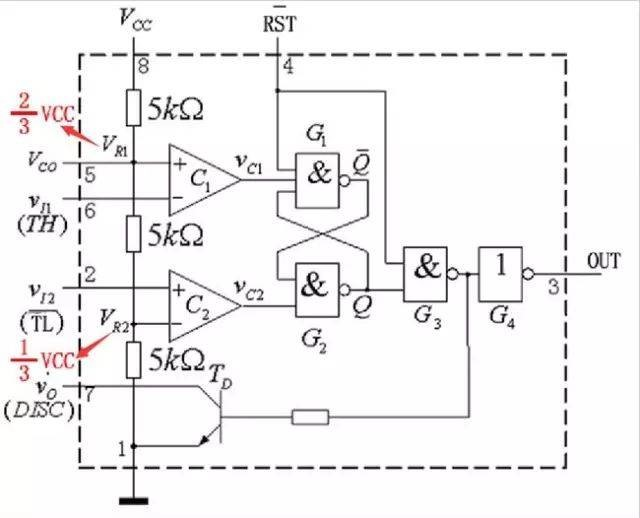
\includegraphics[width=0.45\textwidth]{555in}}\subfigure[555外围电路(采用multisim辅助工具搭建)]{
    \label{555tools}
    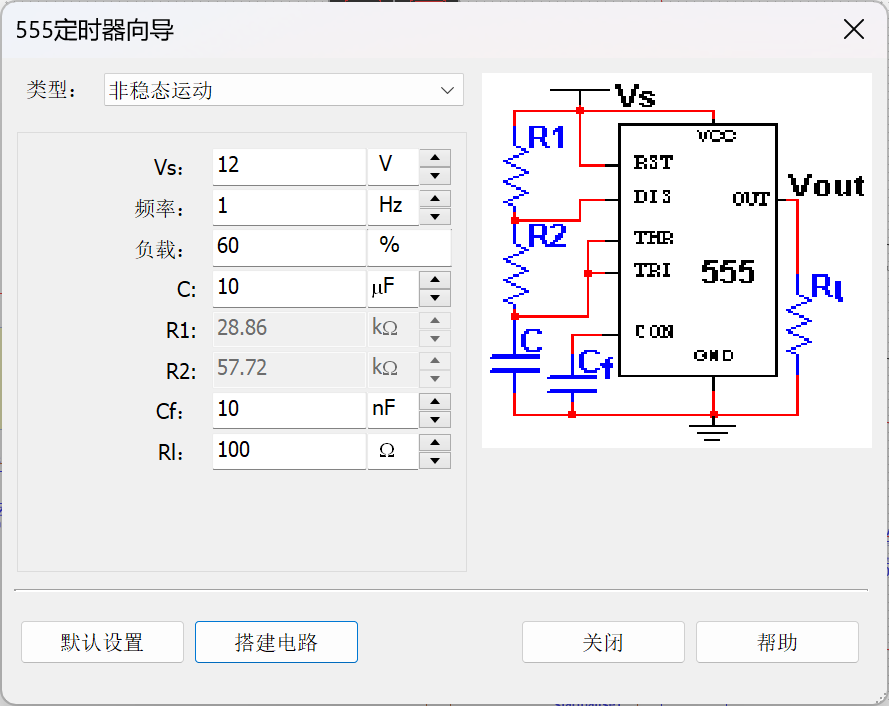
\includegraphics[width=0.45\textwidth]{555tools}}
    \caption{555电路的内部结构及外围电路如图所示}
    \label{555}
  \end{figure}
  \begin{figure}[H]
    \centering  %图片全局居中
    \label{4511BP}
    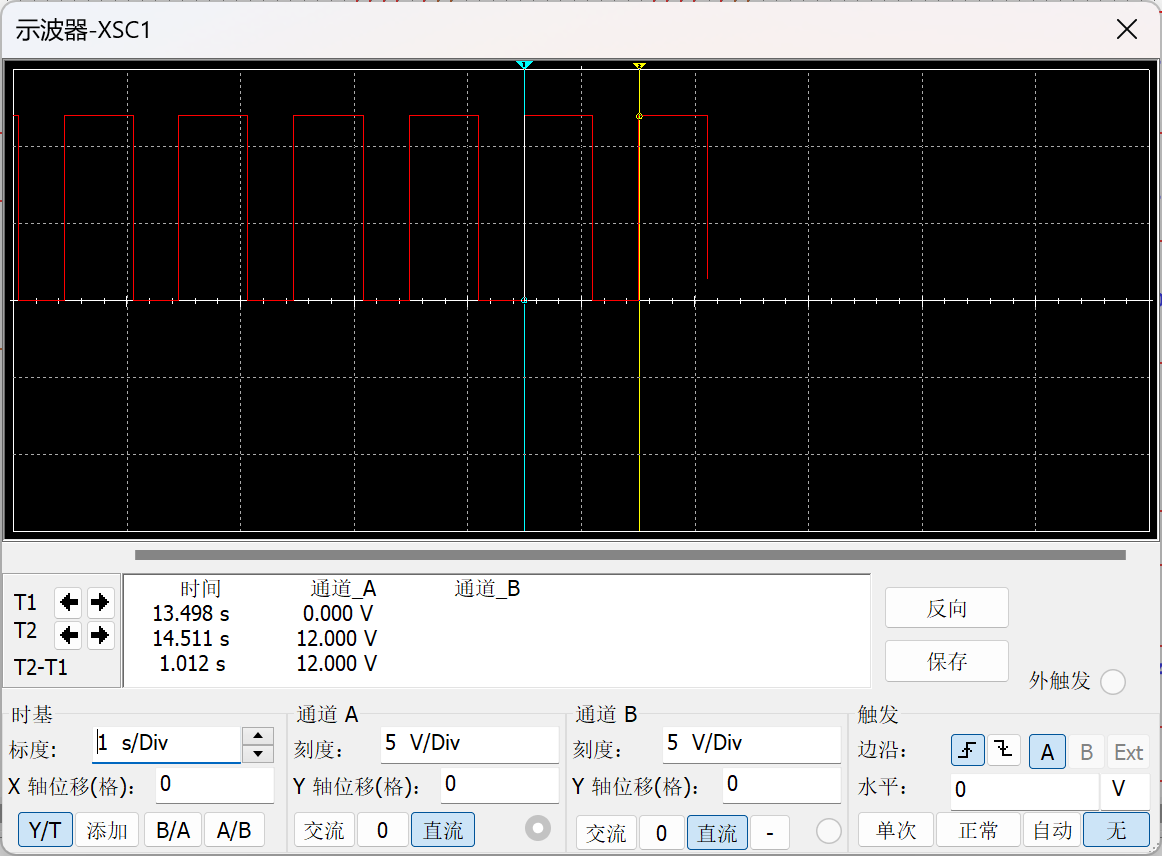
\includegraphics[width=1\textwidth]{sbq.png}
    \caption{555定时器的输出波形}
    \label{4511BP}
  \end{figure}
    
  缺点:电路连接起来比较复杂,而且要求较多,接口也比较复杂。
  \subsection{计数器}
  \subsubsection{计数器选择}
  为了实现递减计时,可以采用74LS190N。74LS190 是一款 4 位二进制可逆计数器,属于 LS 系列集成电路,广泛应用于数字电路中。它能够在时钟信号的控制下进行向上计数或向下计数,且支持同步复位功能,能够将计数值重置为零。该计数器具有四个二进制输出端口,用于显示当前的计数值。通过控制输入端口,用户可以选择计数方向(向上或向下)以及是否启用复位。74LS190 主要用于需要可逆计数的场合,如数字时钟、定时器、事件计数以及频率分频等应用,是一种高效且灵活的计数器解决方案。
  74LS190N的真值表如下:
  \begin{figure}
       \centering
        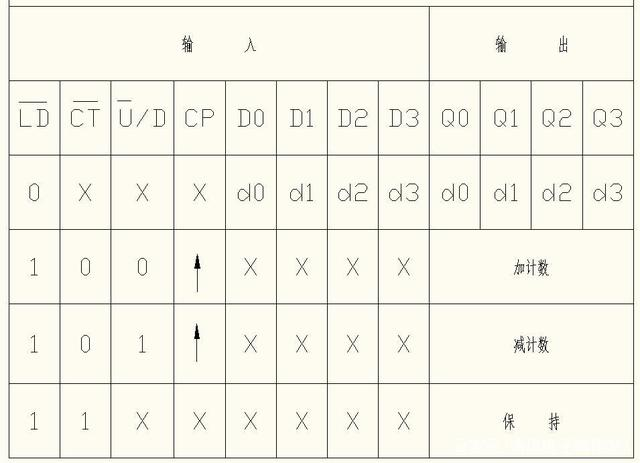
\includegraphics[width=\linewidth]{zzb}
        \caption{74LS190N真值表}
        \label{zzb}
      \end{figure}
      \\[1cm]
  \subsubsection{计数器连接}
  
  模24倒序计数可以采用两片74LS190N级联(将低位芯片的RCO与高位的使能端相连接)实现功能(详细连接图见后文)。
  计数开始前高位芯片置(0010),低位置入(0100)。
  当低位芯片计数到(0000)时,高位芯片计数减1,低位芯片回到(1001),以此类推。
  当计数到(0000,0000)时,计数器停止计数。
 
  \subsection{控制模块}
  \subsubsection{RESET按键}
  控制计时器回到24s,同时暂停报警信号。74LS190N为异步置数,所以将两芯片LOAD端通过弹簧按键与高电平相接,当松开时输入高电平正常计数,按下时输入低电平异步置数复位到24s。
  \subsubsection{START/PAUSE按键}
  为使计数器计时停止计数,采用一个或非门,当一端接入高电平时可以封锁信号源输出的1HZ	信号从而实现暂停计数的目的。分为两种情况暂停:第一种情况为两芯片同时计数到0000时停止计数。可以将其~RCO端通过取反后连接与门作为一个控制开始暂停的或非门的一个输入。第二种情况为按键控制暂停与开始,本设计采用一个D触发器来保存状态,触发器的D端与~Q相接,每输入一个高电平翻转输出Q。所以将按键START/PAUSE与高电平相连。按下奇数次时Q为低电平,信号源可以输入信号到芯片,偶数次时Q为高电平,封锁信号源输出暂停计数。(经仿真测试为了防止复位为24s的瞬间就开始计数按下RESET按键的同时也要向D触发器输送一个高电平来确保D触发器Q为0,不直接开始计数)

  \subsection{报警模块}
  \subsubsection{蜂鸣器介绍}
  蜂鸣器是一种发声器件,广泛应用于电子设备中。蜂鸣器分为有源蜂鸣器和无源蜂鸣器。有源蜂鸣器内部已经集成振荡电路,可以直接供电工作,而无源蜂鸣器需要外部提供振荡信号才能工作。蜂鸣器图如下:
  \begin{figure}[H]
    \centering  %图片全局居中
    \label{蜂鸣器}
    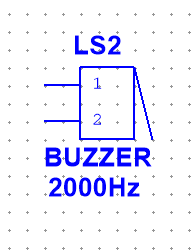
\includegraphics[width=0.35\linewidth]{buzzer.png}
    \caption{蜂鸣器}
    \label{蜂鸣器}
  \end{figure}
  \subsubsection{蜂鸣器连接}
  本设计采用有源蜂鸣器。一端接电源,当两芯片同时计数到0000时向其另一端输入低电平,完成递减到0秒时发出报警信号的功能。当不是0000 0000状态时输出高电平不发出声音。

  \subsection{数码管显示模块}
  \subsubsection{4511BP介绍}
  4511BP 是一个由德州仪器(Texas Instruments)生产的七段显示器驱动芯片,它的主要功能是将二进制编码的十进制数字(BCD)转换为七段显示器的控制信号。4511BP 接受 4 位的 BCD 输入,这些输入值表示数字 0 到 9。根据输入的 BCD 数字,4511BP 控制七段显示器上的相应段的开关状态,进而显示出对应的数字。例如,当输入 0001(BCD 表示数字 1)时,4511BP 会驱动显示器的段,使其显示数字 "1"。该芯片通常用于计数器、数字时钟、仪表等设备中,能够驱动一个或多个七段显示器。4511BP 芯片支持低电压工作,常见的工作电压为 5V,适用于各种电子产品的数字显示部分。它的封装通常为 DIP-16 型,通过与其他逻辑电路配合使用,可以实现更复杂的显示功能。
  \begin{figure}[H]
    \centering  %图片全局居中
    \label{4511BP}
    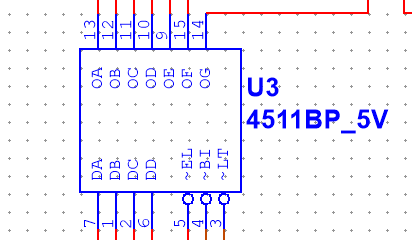
\includegraphics[width=0.45\textwidth]{4511BP}
    \caption{4511BP}
    \label{4511BP}
  \end{figure}
  \subsubsection{4511BP连接}
  4511BP的A、B、C、D输入端分别与74LS190N的输出端相接,将计数器输出的二进制数转换为十进制数,再由4511BP驱动七段数码管显示
  。
  \section{电路图}
  \begin{figure}[H]
    \centering 
    \label{电路图1}
    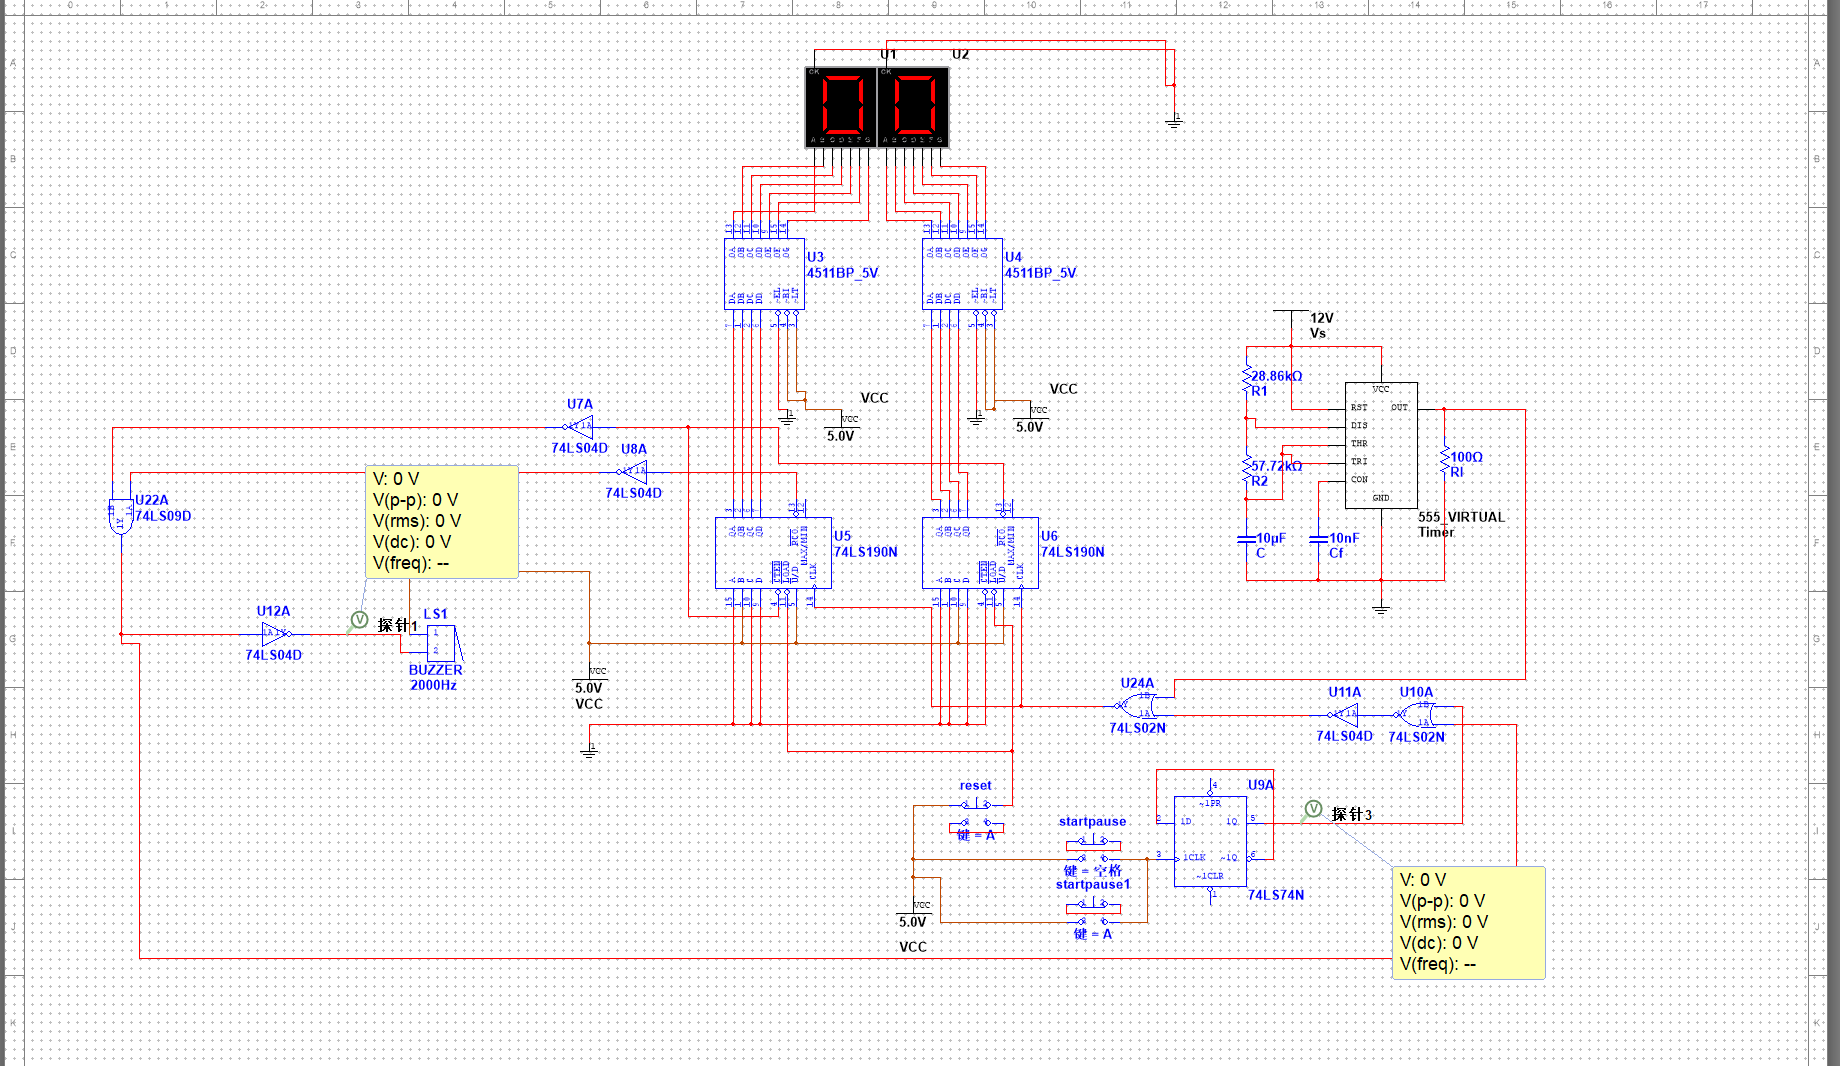
\includegraphics[width=1\textwidth]{1}
    \caption{报警状态}
    \label{电路图1}
    \end{figure}

  \begin{figure}[H]
    \centering  %图片全局居中
    \label{电路图2}
    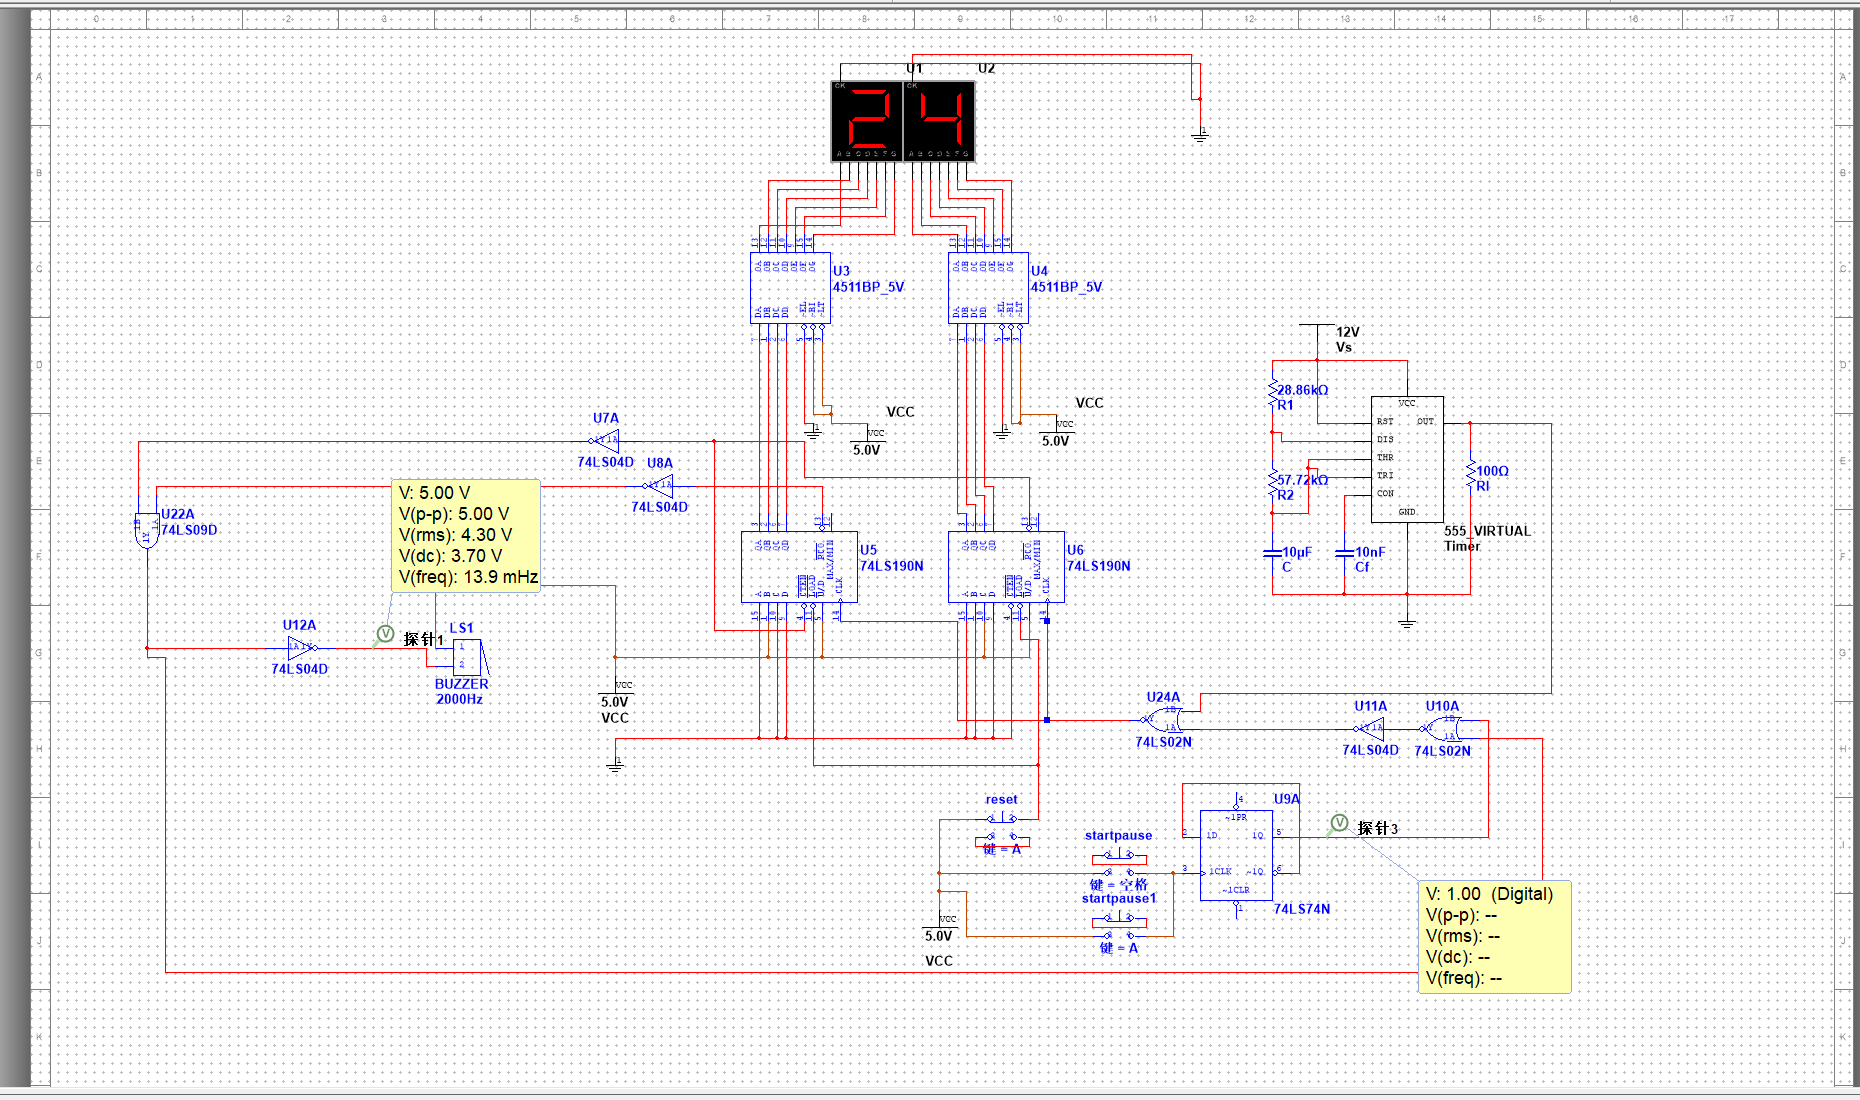
\includegraphics[width=1\textwidth]{2}
    \caption{复位状态}
    \label{电路图2}
  \end{figure}

  \begin{figure}[H]
    \centering  %图片全局居中
    \label{电路图3}
    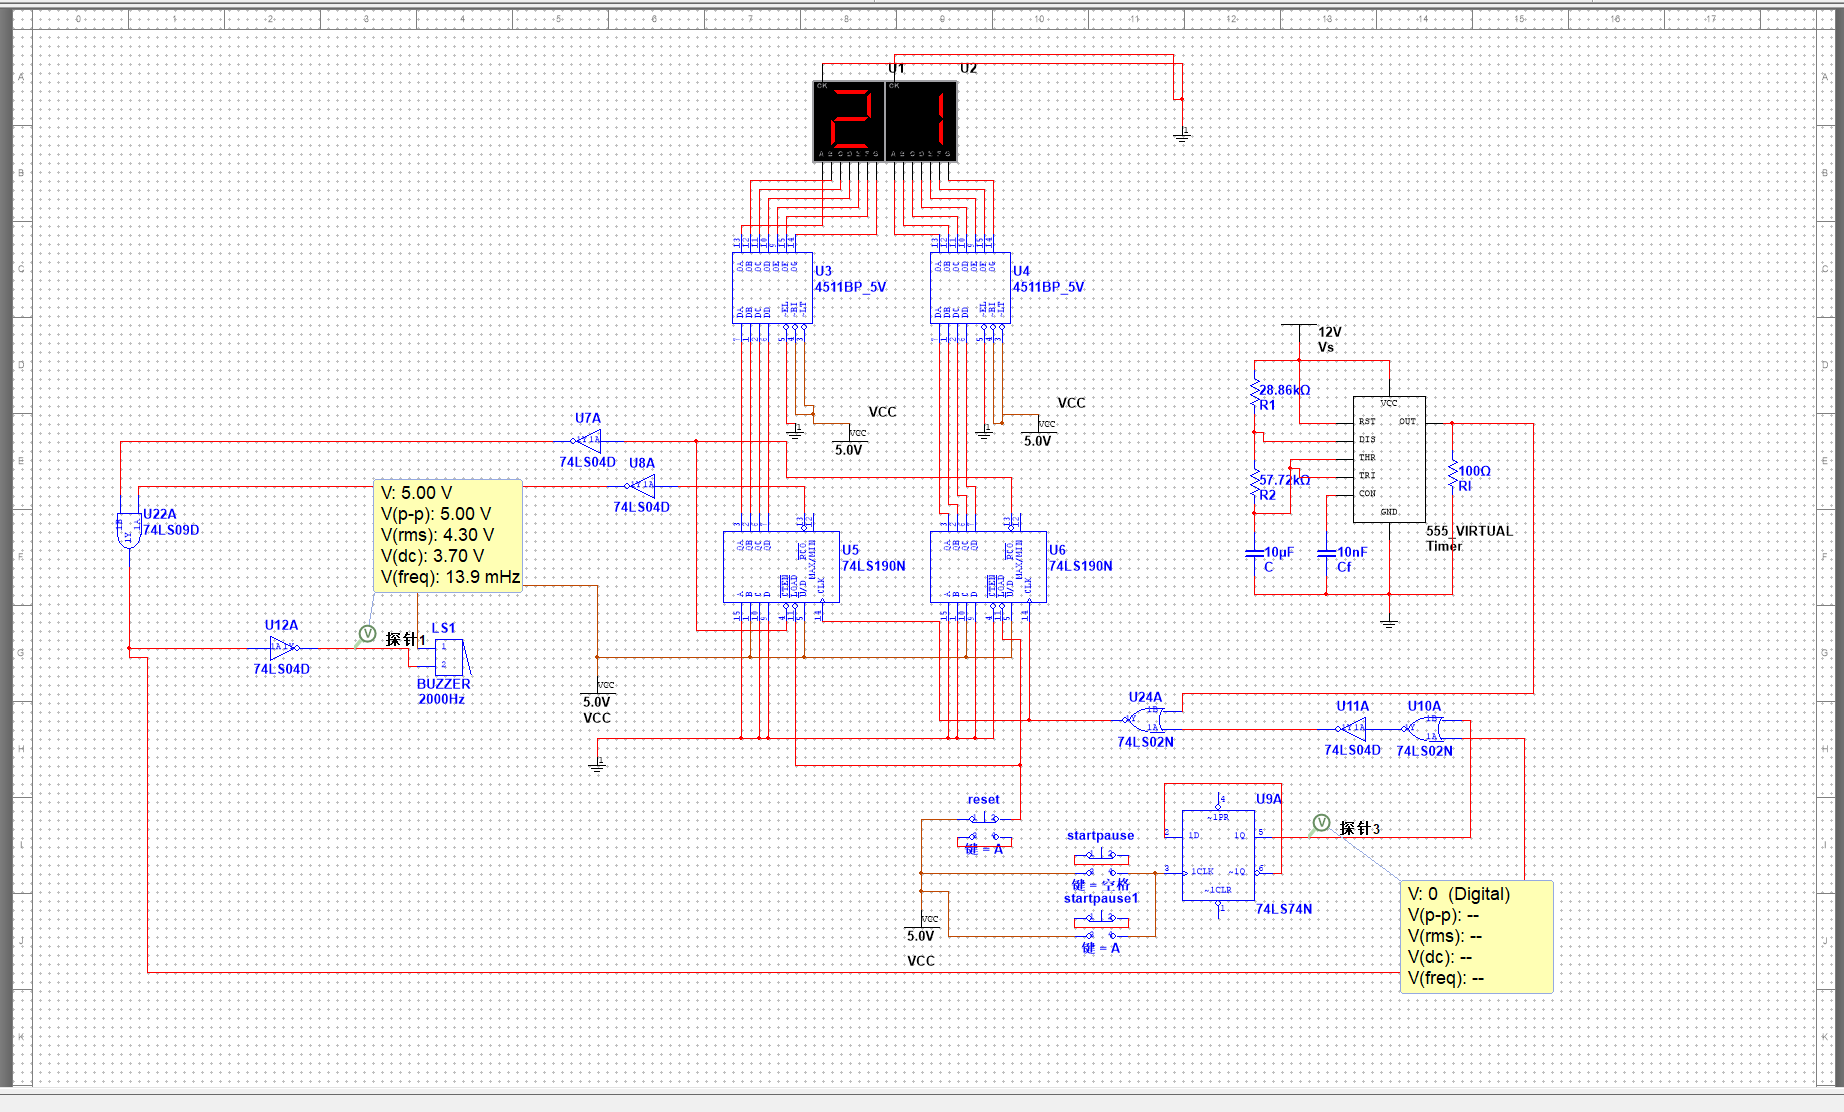
\includegraphics[width=1\textwidth]{3}
    \caption{计时状态}
    \label{电路图3}
  \end{figure}

  \begin{figure}[H]
    \centering  %图片全局居中
    \label{电路图4}
    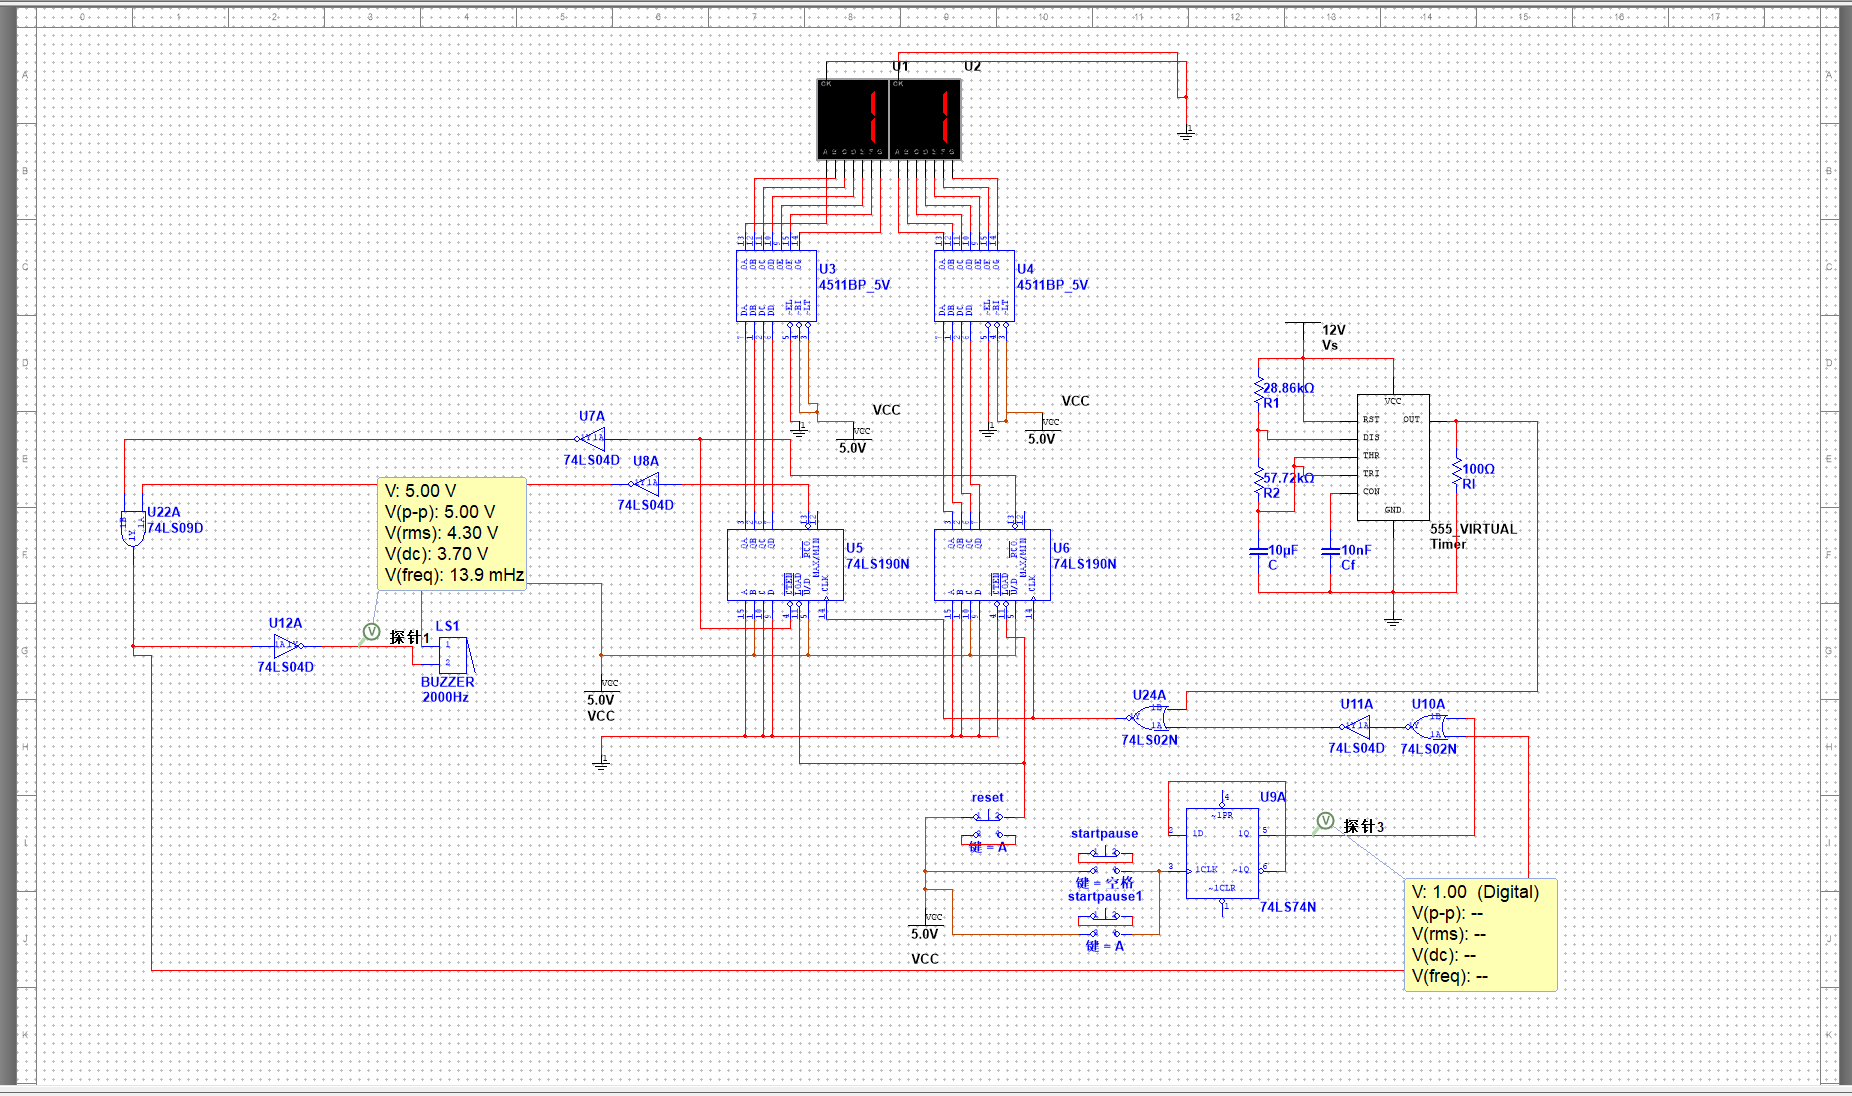
\includegraphics[width=1\textwidth]{4}
    \caption{暂停状态}
    \label{电路图4}
  \end{figure}

  


  \section{实验总结}
  通过完成此次篮球竞赛24秒计时器的设计,我对数字电路和逻辑设计有了更深入的理解和实践体验。在设计过程中,我主要收获了以下几点心得:\\
1.	模块化设计的重要性
本次设计任务较为复杂,需要实现24秒倒计时、外部控制以及报警功能。因此,我将整个设计划分为计时器模块、控制模块、数码管显示模块和报警模块。这种模块化设计思维不仅使问题分解得更清晰,也大大提高了电路设计的可维护性和可调试性。在今后的实际工程设计中,模块化思想依然是值得推崇的设计方法。
\\2.	器件选型与应用技巧
我选择了74LS190N作为核心计数器,该芯片的同步递减计数功能完美符合设计需求。同时,为了实现秒级递减计时,我结合了555定时器生成1Hz的时钟信号。在此过程中,我深刻体会到合理选用芯片和器件的重要性,不仅要满足功能需求,还要简化电路结构,减少冗余设计。
\\3.	控制逻辑的实现与挑战
在设计控制模块时,如何实现按键控制的启动、暂停与清零功能是一个较大的挑战。通过引入D触发器来存储状态并与按键结合,我成功实现了按键翻转控制的功能。同时,为了防止计时器复位后立即开始计数,我在RESET按键上加入了信号同步处理。这一部分让我对控制逻辑的实现有了更深的理解,并提高了对触发器和按键消抖等技术的掌握。
\\4.	仿真验证的实践经验
在完成电路设计后,我利用仿真工具验证了电路的功能,包括正常计时、暂停、复位及报警等状态。通过仿真,我能够迅速发现设计中的不足并及时进行调整。这让我意识到仿真工具在电路设计中的关键作用,它可以大幅减少设计错误,提高设计的可靠性。
\\5.	理论与实践的结合
此次设计充分将课堂所学的数字电路理论知识与实际应用相结合,使我对二进制计数器、时钟信号生成、逻辑控制等知识点有了更加直观和深入的理解。特别是在应用过程中,我加深了对基本芯片功能和电路原理的记忆,并培养了解决实际问题的能力。

通过这次综合作业的设计,我不仅提升了自身的数字电路设计技能,还学会了如何从整体上把握一个项目的设计流程。未来,我将继续通过更多实践项目来巩固和扩展自己的知识和能力。

\end{spacing}
\end{document}


 